\label{sec:mcnp}
\section{MCNP}
\subsection{General information}
MCNP, or Monte-Carlo N-Particle Transport Code, is a software package that is used for nuclear simulations. It is based on Fortran, the most common version being Fortran-90. A typical MCNP program contains definitions for geometries in a 3D dimensional Cartesian coordinate system, which are composed of cells, surfaces and their material definitions. In figure \ref{fig:regions}, A and B are two surfaces defined in MCNP. Each surface has a negative and positive value, which is important for particle interaction. If a value is negative, then the surface is facing inwards relative to the origin. The mathematical depiction can be seen in figure \ref{fig:planes}, where the normal vector $n_2$ is expressed by a negative surface number, whilst the vector $n_1$ is a positive surface number.
\begin{figure}[!htbp]
\caption{Normal vectors to a plane.}
\label{fig:planes}
\centering
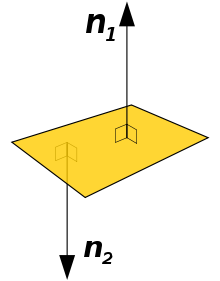
\includegraphics[width=0.25\textwidth]{normals.png}
\end{figure}
Surfaces can be combined together to create cells. Defined as either unions or intersections, the resulting cells from surfaces A and B are seen in figure \ref{fig:regions}. An important MCNP concept to remember is that when looking at a typical geometrical shape, for example a cube, one must double the number of faces. In a cube, the number of faces is 6, however, because of positive and negative surfaces, the shape should be looked at as having 12 faces. Understanding this was a key point in the project. Being able to identify which regions were required and which surfaces to ignore allowed us to carry out simulations more effectively and accurately.
\begin{figure}[!htbp]
\caption{Example MCNP regions.}
\label{fig:regions}
\centering
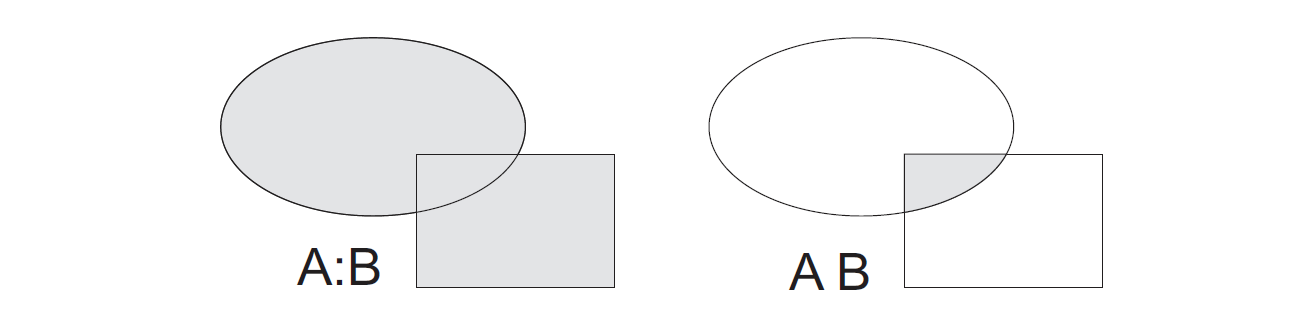
\includegraphics[width=0.75\textwidth]{regions.png}
\end{figure}
A sample MCNP input file consists of the following components. There are 3 blocks, each separated by a blank line: first come the cell definitions, followed by surface definitions and finally the data blocks (introduced in section \ref{sec:simulations}). There are also optional comments that can be added at different points. The blank lines, however, need to be kept, otherwise MCNP will not be able to distinguish the blocks. A full line comment starts with the letter "c", whilst an inline comment starts with a dollar sign (\$). It is important to note that all lines should not exceed 80 characters in length. A visual representation of an MCNP program can be see in figure \ref{fig:program}
\begin{figure}[!htbp]
\caption{MCNP program structure.}
\label{fig:program}
\centering
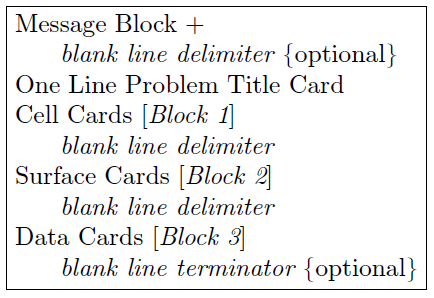
\includegraphics[width=0.75\textwidth]{prog.png}
\end{figure}
\subsection{Example geometry}
A good way to understand MCNP syntax and its complexity is a simple example. As a result, a cube will be submerged into a spherical container and that container will be filled with water. Throughout the project, it was found that specifying surfaces first was an easier approach, followed up the cell definitions. As a result, the input file was structured out of order, however, this allowed for a more step-by-step approach to the simulation setup. In order to create a cube, the general procedure is the following:
\begin{enumerate}
	\item Specify 6 outward facing surfaces.
	\item Specify 6 inward facing surfaces.
	\item Combine all of the relevant surfaces into a cell. For example, the outside of the cube would be a union of the outward facing surfaces, and the inside will be a union of the inward facing ones.
\end{enumerate}
Although this is only 3 steps, the procedure is fairly complex. In order to specify a single surface of a cube, one must figure out the side length, center and boundaries of the square in question. Doing this 12 times in a 3D coordinate system becomes monotone and challenging, especially when dealing with complex, irregular geometries. MCNP does have a solution, however - macrobodies. With one command, MCNP will know that the shape specified is a cube, sphere or pyramid (to name a few). The command for a rectangular parallelepiped is \textbf{RPP}. In order to create a cube centered at the origin with a side length of $10$cm, the command is:
\begin{center}
\begin{tabular}{c}
\begin{lstlisting}
10 RPP -5 5 -5 5 -5 5
\end{lstlisting}
\end{tabular}
\end{center}
In the above example, 10 is the number of the macrobody, which will be important in the cell block. The first two numbers indicate a starting and ending x-coordinate\footnote{MCNP units are metric, with length defaulting to centimeters.}, followed by the same syntax for a y and z coordinate. The next step is to add a container around the cube. This can be a sphere, again, specified by a macrobody, the command for which is \textbf{SO}. If the radius is set to 100cm, then:
\begin{center}
\begin{tabular}{c}
\begin{lstlisting}
20 SO 100
\end{lstlisting}
\end{tabular}
\end{center}
The structure is similar - 20 is the label for the macrobody, SO is the command, 100 is the radius.
%Criticalities, data blocks, random walks are all here.
\label{sec:simulations}
\subsection{Simulations}


%In order to demonstrate the concept, one can look at a cube. A cube has 6 surfaces, however, in MCNP, one can specify negative and positive values for these surfaces, so the actual number of surfaces is 12 for a cube.

%Particle simulation section
%A good way to look at an example particle simulation is the random walk problem, the diagram for which can be seen in figure \ref{fig:randomwalk}.
% \begin{figure}[!htbp]
% \caption{MCNP random walk.}
% \label{fig:randomwalk}
% \centering
% 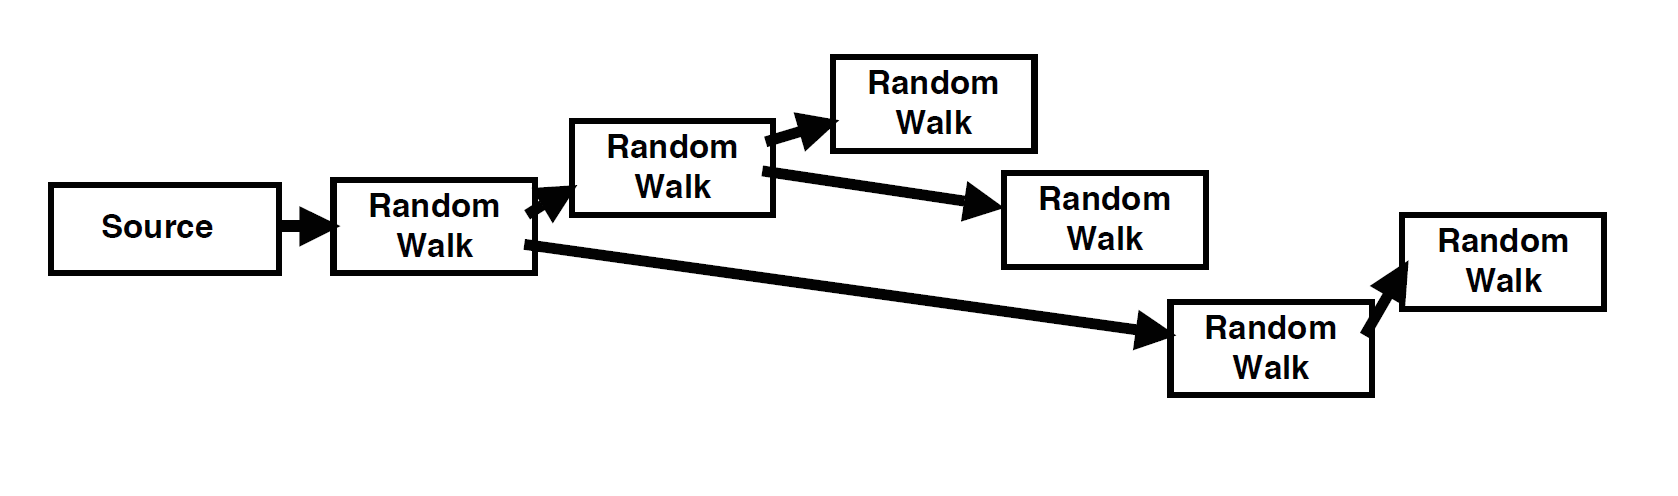
\includegraphics[width=0.75\textwidth]{walk - edited.png}
% \end{figure}
% In the diagram, some particle (a proton or a neutron, for example) starts its path at the source block and is launched in a random direction. After that, it can interact with something else in the simulation space - other protons or neutrons. A collision takes place and the particle is launched into another random direction. This goes on for a certain number of cycles, specified by the user.

%takes Monte-Carlo simulations one step forward. The program solves a series of random-walk problems. In the current case, a random particle is traced from its source to a certain definition.